%!TEX TS-program = pdflatex
\documentclass[12pt]{article}  % larger font to compensate for long lines with fullpage
\usepackage{ifpdf,ifxetex}

\ifxetex
% \usepackage{fontspec}
\else % inputenc is incompatible with xetex (which always takes UTF-8 as input)
\usepackage[utf8]{inputenc}
\fi
\usepackage{ifthen}
\usepackage{graphicx}
\usepackage[pdfborder={0 0 0}]{hyperref} % use hyperref without borders
\usepackage{url}
\usepackage{authblk}

% Template for GWD/GFD documents.
% Created by Freek Dijkstra, original concept by Bruce Lowekamp.
% This template is placed in the public domain.

% Define some basics for your document:

\title{Describing a monitoring infrastructure with an OCCI-compliant schema}  % Full title of the document
\newcommand{\shortdoctitle}{OCCI Monitoring}  % Title used in page header
% \date{} and \author{} are currently ignored
\newcommand{\authorsshort}{Augusto Ciuffoletti, Dept. Of Computer Science - Univ. of Pisa}  % name(s) and institution(s) of corresponing author(s) as shown on the title page.
\newcommand{\publicationdate}{February 2013}  % Date of first publication of the document
% \newcommand{\revisiondate}{December 2010}  % Optional: date of last revision of the document
\newcommand{\copyrightyears}{2012-2015}  % Years used in copyright notice
\newcommand{\docseries}{GWD-C-P}  % GWD-R, GWD-I or GWD-C (for working drafts), GFD-I, GFD-R, or GFD-C
\newcommand{\groupname}{OCCI-WG}  % Optional: name of the authoring working or research group
\newcommand{\groupurl}{\href{mailto:augsuto@di.unipi.it}{augusto@di.unipi.it}}  % Optional: URL or email address of the authoring working or research group
\newcommand{\documenturl}{}  % Optional: URL of this document


% Read pictures from img/ and current directory
\graphicspath{{img/}{./}}

%%% GWD/GFD header follows %%%
% Feel free to make changes, as long as your document follows the guidelines of GFP.152

%\usepackage[numbers]{natbib} % Use [1] for references, 
%\usepackage[authoryear]{natbib}
\bibliographystyle{plainnat} % References show full author name(s) and document URL
\usepackage[sf,compact]{titlesec} % Use sans-serif for section headers

\usepackage[titles]{tocloft} % Format table of contents
% (tocloft is used, since titletoc is incompatible with xetex.)
\renewcommand{\cftsecfont}{\sffamily}
\renewcommand{\cftsubsecfont}{\sffamily}
\renewcommand{\cftsubsubsecfont}{\sffamily}
\renewcommand{\cftsecpagefont}{\sffamily}
\renewcommand{\cftsubsecpagefont}{\sffamily}
\renewcommand{\cftsubsubsecpagefont}{\sffamily}
\renewcommand{\cftsecleader}{\cftdotfill{\cftsubsecdotsep}} % dots for sections the same as for subsections
\setlength{\cftbeforesecskip}{0.5ex}


\usepackage{parskip} % Blank lines between paragraphs, no indentation.

% % Tune placement of figures. (defaults are so strict that images and text are often separated.)
% \renewcommand{\textfraction}{0.05}  % min fraction of page for text. default: 0.2
% \renewcommand{\topfraction}{0.95}   % max fraction of page for floats at top. default: 0.7
% \renewcommand{\bottomfraction}{0.95}% max fraction of page for floats at bottom. default: 0.3
% % \renewcommand{\floatpagefraction}{0.35} % min fraction of floatpage that should have floats. default: 0.5
% % \setcounter{totalnumber}{5}         % max number of floats on a page
% 
% % Tune placement of text. (defaults are not strict enough.)
% \widowpenalty=500% penalty for single line on top of succeeding page. default 150
% \clubpenalty=500% penalty for single line on bottom of preceeding page. default 150
% \tolerance=1000% abort if the penalty exceeds 1000. default infinite.

% font style for text body
% \renewcommand{\familydefault}{\sfdefault}

% font style for headers and footers
\newcommand{\headerstyle}{\sffamily} % sans-serif

% Set page margins
\usepackage{fancyhdr}
\addtolength{\headheight}{15pt}
\renewcommand{\headrulewidth}{0pt}
% \setlength{\headrulewidth}{0pt}
\setlength{\headsep}{20pt}
\usepackage[headings]{fullpage}  % small margins

% Macro to check if (optional) values above are defined or not.
\newcommand{\ifnonempty}[2]{\ifthenelse{\isundefined{#1}}{}{\ifthenelse{\equal{#1}{}}{}{#2}}}

% Define page header and footers
\pagestyle{fancyplain}
\fancyhf{}
\lhead{\fancyplain{}{\headerstyle\docseries}}
% use \revisiondate if defined, otherwise \publicationdate for right header:
\rhead{\fancyplain{}{\headerstyle\ifthenelse{\isundefined{\revisiondate }}{\publicationdate}{\ifthenelse{\equal{\revisiondate}{}}{\publicationdate}{\revisiondate}}}}
\lfoot{\headerstyle\ifnonempty{\groupurl}{\groupurl}}
\rfoot{\headerstyle\thepage}
\thispagestyle{plain}

\begin{document}

% Title page header
{\noindent
\begin{minipage}[t]{3.0in}
\headerstyle
\docseries \\
\ifnonempty{\groupname}{\groupname \\}
\ifnonempty{\groupurl}{\groupurl \\}
\ifnonempty{\documenturl}{\documenturl \\}
\end{minipage}
\hfill
\raggedleft
\begin{minipage}[t]{3.0in}
\raggedleft
\headerstyle
\authorsshort \\
\publicationdate \\
\ifnonempty{\revisiondate}{Revised \revisiondate \\}
\end{minipage}
}

% My commands!

% This is for signed remarks
%\newcommand{\rem}[2]{\footnote{{\bf Remark by #1}: #2}}
\newcommand{\rem}[2]{}

\newcommand{\attributes}[2]{
\begin{tabular}{llll|p{7cm}} \hline
\multicolumn{4}{l}{Set of Attributes for the {\em #1}} \\ \hline
name & type & mutable & required &  Description \\ \hline
#2 \hline
\end{tabular}
}
\newcommand{\oc}[0]{\tt OCCI}
\newcommand{\mi}[0]{{\em Mix-in}}
\newcommand{\rs}[0]{{\em Resource}}
\renewcommand{\ln}[0]{{\em Link}}
\newcommand{\sens}[0]{{\em Sensor Resource}}
\newcommand{\tool}[0]{{\em Tool}}
\newcommand{\comp}[0]{{\em Compute}}
\newcommand{\coll}[0]{{\em Collector Link}}

\newcommand{\resource}[2]{
\begin{tabular}{ll}
\hline
Model attribute & value \\ \hline
scheme & http://ogf.schemas.sla/occi/monitoring\# \\
term & #1 \\
attributes & #2 \\
related & http://ogf.schemas.sla/occi/core\#resource \\ \hline
\end{tabular}
}

\newcommand{\link}[2]{
\begin{tabular}{ll}
\hline
Model attribute & value \\ \hline
scheme & http://ogf.schemas.sla/occi/monitoring\# \\
term & #1 \\
source & URI \\
target & URI \\
attributes & #2 \\
related & http://ogf.schemas.sla/occi/core\#link \\ \hline
\end{tabular}
}

\newcommand{\mixin}[2]{
\begin{tabular}{ll}
\hline
Model attribute & value \\ \hline
scheme & http://ogf.schemas.sla/occi/monitoring\# \\
term & #1 \\
attributes & #2 \\ \hline
\end{tabular}
}

\newcommand{\extramixin}[2]{
\begin{tabular}{ll}
\hline
Model attribute & value \\ \hline
scheme & http://provider.com/monitoring\# \\
term & #1 \\
attributes & #2 \\ \hline
\end{tabular}
}
% End of my comments

\begin{center}
\makeatletter
\Large\bf\textsf \@title
\makeatother
\end{center}


%%% End of header, insert content below this line %%%

\subsection*{Status of This Document}

% Pick one of the following:
Group Working Draft (GWD)
%Grid Final Draft (GFD)
%Grid Recommendation
%Obsolete. This document is replaced by/obsoleted by GFD-I.xxx~\cite{gfd0000}.
%Historical

%\subsection*{Obsoletes}
%% include or remove this section if applicable

%This document obsoletes GFD-I.xxx~\cite{gfd0000}.

\subsection*{Document Change History}
%% include or remove this section if applicable

February 1st 2013: first revision (Augusto Ciuffoletti)

\subsection*{Copyright Notice}

Copyright \copyright \ Open Grid Forum (\copyrightyears).  Some Rights Reserved.  
Distribution is unlimited.

\subsection*{Trademark}
%% include or remove this section if applicable

OCCI is a registered trademark and service mark of the Open Grid Forum. 

\phantomsection\addcontentsline{toc}{section}{Abstract}
\section*{Abstract}

This document {\em provides information} to the Grid community about resource monitoring. It {\em describes} an OCCI Extension that allows to inspect the operation of functional resources; the provision of this API is considered as optional for the provider.

This document {\em presents} two further {\em Kinds}: the \sens, that processes metrics, and the \coll, that extracts and transports metrics. They are defined as generic {\em Kinds}, that need to be specialized using OCCI \mi s. Using this API, the user is provided with a monitoring infrastructure {\em on demand}.

This document does not define any standards or technical recommendations.

One relevant target of this document is to provide a building block for the design of an API for Service Level Agreement (SLA): under this light, the API for the Resource Monitoring Infrastructure offers the tools to verify and implement the Service Level Objectives (SLO).

\phantomsection\addcontentsline{toc}{section}{Contents}
\tableofcontents

\newpage

\section{Introduction}

This document describes an interface to define a monitoring infrastructure. It is based on the concepts introduced by OCCI, it is intended to be a first step towards the definition of a protocol to manage and verify Service Level Agreement (SLA), not being limited to SLA.

The purpose of this specification is that of giving the user the possibility to arrange a monitoring infrastructure in the way that best suits user's needs, instead of limiting the user to the implicit monitoring provided by a SLA. The existence of a standard specification makes it possible for the user to manage distinct cloud providers, possibly at the same time, using the same interface.

The importance of a configurable monitoring infrastructure emerges specifically in complex scenarios, where the user is in fact an intermediate service provider, that provides SLA services to third party users: in that case, the intermediate provider may decide to provide SLA options that differ from that of the low level provider, and therefore to perform specific measurements on the infrastructure leased by the low level provider(s).

The management capabilities should also extend to the adaptive, and dynamic configuration of the components that contribute to the monitoring activity: the specification schema must give the user the possibility to explore the available functionalities in order to adaptively arrange a monitoring infrastructure, and to modify them according with changing needs.

One relevant fact about monitoring infrastructures is that it is extremely difficult to give a {\em detailed} framework for them that extends its validity to any reasonable use case or provider. The reason is that each use case and provider exhibits local variants that do not fit a rigid {\em standard} approach. Also, the metrics that are used to evaluate the performance of the system are many, and subject to continuous changes due to the introduction of new technologies. Thus we have made an effort to introduce a generic schema that can be adapted to effectively describe the relevant aspects of a monitoring infrastructure, but that does not interfere with details that depend on the specific environment.

The OCCI Core Model \cite{occi:core} is well suited for the task, since it embeds the tools needed to extend a framework with provider specific details: this enables the specification of the abstract model, leaving to the user the task of making explicit the details, targeting a specific provider or technology. Furthermore, we claim that the specifications given in this document can find an application in environments other than computing infrastructures, since we abstract from the details that characterize cloud infrastructure resources.

The approach followed in this document is similar to that found in the infrastructure document (GFD-P-R.184 \cite{occi:infr}): the monitoring capability is associated with a new {\em Kind}, the {\em Sensor}, that is related with the OCCI Core Model Resource type. A \sens\ instance is a black box that collects metrics from its input side, and delivers aggregated metrics from its output. The input and output channels are modeled with another {\em Kind}, called {\em Collector}, that is related with the OCCI Core Model Link type. The role of a \coll\ instance is twofold: on one side it indicates the way metrics are conveyed to the target \rs, on the other it indicates a specific monitoring technique applied on the source \rs. Both capabilities are controlled with \mi\ association. For instance, the provider may offer the client a specific {\em Ping Mixin} that can be associated with a \coll\ originating from a {\em Network Resource}: such a configuration will deliver metrics like the roundtrip time and the packet loss rate to the attached \sens. To enable the discovery of such \mi s, they are gathered under specific collections.  

Using these basic building blocks the designer is able to assemble complex, multilayer monitoring infrastructures: for instance, a \sens\ can be used to aggregate a storage throughput using the input from three \coll s, one for the average response time, one for the mean time between failures, and another for network delay, and provide the results to an upstream \sens\ that aggregates the same results from other \sens s. On the other hand, the model is able to describe very simple scenarios, like a compute \rs\ that logs its activity in a database hosted by a storage \rs: in that case one \coll\ connects the compute resource to the storage, without the need of a \sens. Appropriate \mi s associated with the \coll\ describe the logging activity and the database access mode.
\rem{author}{Why not a mixin to the monitored resource directly? I envision problems emerging with the implementation. A resource can be ``prepared'' for monitoring, but the way in which the Monitoring Link will interact with such preparation is not clear. In addition, consider that the same tool might be the target of several links, with distinct configuration parameter. How can the control parameters of the mixin be exposed in such a case? Instead, if the mixin is embedded in the link, it is the responsibility of the link implementation to configure it, and to couple it with the publishing technology indicated in the link}

Note that the schema is transparent, in particular, to the existence of a standard for metric identifiers: if one exists, the interoperability of distinct monitoring infrastructures is certainly improved. We consider that the user that interacts with the monitoring infrastructures either knows about the identifiers used by the provider, or uses an interface (e.g., a SLA negotiation service) that translates provider specific identifiers into interoperable ones. This document highlights further standardization issues.

Summarizing, the specification introduced in this document requires that the conformant provider implements two {\em Kind}s: the {\em Sensor Resource} and the {\coll. Three tagging \mi s are also defined, namely {\em ToolSet}, {\em CollectorSet} and {\em AggregatorSet}, to identify the collection of mixins that describe the specific capabilities associated with an instance of the above {\em Kind}s. 

\subsection{Terminology shortcuts}

To distinguish a {\em Resource} instance from its {\em Kind}, we will use the indeterminative article for the instance (e.g., ``a \rs''), and the determinative article for the {\em Kind} (e.g., ``the \rs''). The plural is reserved to instances (e.g., ``the \rs s''). In case of ambiguity we will further specify ``instance'' or ``{\em Kind}''. 

We will use the term {\em $<$mixin id$>$ collection} to indicate the set of \mi s that are associated with the identified tagging \mi. The provider ensures that the \mi s in a given collection have defined semantics, as explained in the rest of this paper. 

\section{Specification of the compliant server}

The compliant server MUST define the following {\em Kind}s:

\begin{description}

\item [\sens] that describes how monitoring results are aggregated (see table  \ref{tab:sensor});

\item [\coll] that describes how monitoring results are trasferred between {\em Resource}s (see table \ref{tab:collector});

\end{description}

In addition, the compliant server MUST define the following {\em Mixin}s (see table \ref{tab:mixin}): 

\begin{description}

\item [{\em AggregatorSet}] that is used to tag the \mi s describing the aggregation function operated by a \sens;

\item [{\em ToolSet}] that is used to tag \mi s describing Monitoring tools associated with a \coll;

\item [{\em CollectorSet}] that is used to tag the \mi s that describe the technique used to transport monitoring results in a \coll;

\end{description}

\begin{table}
\scriptsize
\mixin{sensor\_tpl}{None}

\mixin{tool\_tpl}{None}

\mixin{publish\_tpl}{None}

\caption{Definition of the template \mi s \label{tab:mixin}}
\end {table}


\subsection{The \sens \label{sec:sensor}}

\begin{table}
\scriptsize
\resource{\sens}{(see below)}

\attributes{Sensor Resource}{
occi.sensor.period & number & true & true & The time between two following measurements \\
occi.sensor.periodspec & string & true & false & granularity, accuracy, exponent of period measument \\
occi.sensor.timebase & number & false & true & The server time when the timestart and timestop are modified \\  
occi.sensor.timestart &	number & true & true & The delay after which the session is planned to start \\
occi.sensor.timestop & number	& true & true & The delay after which the session is planned to stop \\
occi.sensor.timespec & string & true & false & granularity, accuracy, exponent of time measurement \\
}
\caption{Definition of the {\em Sensor Resource} Kind \label{tab:sensor}}
\end {table}


The \sens\ (see table \ref{tab:sensor}) models the manager of a monitoring activity that encompasses the collection of measurements, their aggregation in composite metrics, and their delivery to the user.

A \sens\ is characterized by attributes that define the rate with which new observations are produced, and by the scheduling times of its operation. The attributes with \verb|required=true| MUST be assigned a legal value upon instantiation. The server MUST reject an incomplete instantiation.

The execution rate is defined using three attributes: the rate itself, and an optional definition of the quality of the timing. This latter attribute contains a triple of numbers encoded as a string, that define the granularity with which the rate is measured, and the accuracy of rate measurement, and the floating point exponent. By default \verb|periodspec="NaN, NaN, 0"|.

The activation of a \sens\ is controlled by two attributes that describe the scheduling of sensor activity: to schedule the execution of a sensor the user modifies the {\tt starttime} with a value indicating how far in the future the instance is going to start its activity. A value of zero corresponds to the immediate start. The server sets the {\tt timebase} attribute corresponding to the reference time of the start time.

All time values are represented as numbers. The {\tt timebase} corresponds to Unix seconds, all timing values use a floating point notation. Also for time values there is a {\tt timespec} attribute analogous to {\tt periodspec}.

\subsection{The \mi\ in the {\em AggregatorSet} collection}

A \mi\ instance in the {\em AggregatorSet} collection is meant to implement the computation of an aggregated metric starting from raw metrics: it represents the function applied by a \sens. In principle, each provider has a distinct offer of such \mi s, so here there is ground for further standardization. If the provider does not adhere to a defined standard, it MUST give an exhaustive documentation of the aggregation functions associated with a \mi.

The attributes of a \mi\ in the {\em AggregatorSet} collection are divided into three groups:

\begin{itemize}
\item Input attributes: they bind a metric in the scope of the \sens\ with an input of the aggregating function. The scope of a \sens\ consists of the {\tt name}s of all the metric attributes of the incoming \coll s. A metric indicated as the value of an input attribute MUST be in the scope of the \sens . For instance, a \sens\ that implements a EWMA may have an {\tt input} attribute equal to 
\begin{verbatim}
data="com.provider.monitoring.collector1.roundtrip"
\end{verbatim}
where \verb&roundtrip& is a metric delivered by an incoming \coll\ {\tt collector1}.
\item Control attributes: they control the operation of the aggregating function (for instance, the gain of an EWMA);
\item Metric attributes: they correspond to the metrics delivered through the outgoing \coll.
\end{itemize}

To enable interoperabilty, the provider SHOULD follow a defined standard for the naming of input, control and result attributes, but its specification falls outside the scope of this document.

\section{The \coll}

\begin{table}
\scriptsize
\link{\coll}{(see below)}

\attributes{Collector Link}{
occi.collector.period & number & true & true & The time between two following measurements \\
occi.collector.periodspec & string & true & false & granularity, accuracy, exponent of period measument \\
}
\caption{Definition of the \coll\ Kind \label{tab:collector}}
\end {table}


The \coll\ models  (see table \ref{tab:collector}) the transfer of metric measurements from one \rs\ to another. The transfer may be motivated, for instance, by the existence of specialized \rs s, by administrative reasons, or to cross inter-provider boundaries.

A \coll\ is characterized by two aspects: one is the activity that extracts metric measurements from the source \rs, and the other is the transport of the measurements to the target \rs. Both of them are defined by \mi s, respectively from the {\em ToolSet} and from the {\em CollectorSet} collections.

Regarding the presence of an associated \mi\ in the above collections, we distinguish two basic cases:

\begin{itemize}

\item if the {\tt target} of the \coll\ is a \sens, then {\em CollectorSet} \mi s SHOULD NOT be associated with the \coll\ instance, and the provider has enough information to implement an appropriate channel;

\item if the {\tt source} of the \coll\ is a \sens, then {\em ToolSet} \mi s SHOULD NOT be associated with the \coll\ instance, since it is considered as not meaningful to monitor a \sens.

\end{itemize}

The metric attributes of the \mi s associated to the \coll\ contribute to the scope of the target \sens\ referenced in sect. \ref{sec:sensor}.

\subsection{The \mi\ in the {\em ToolSet} collection}

The measurement activity is integrated in the \coll\ using a \mi\ in the {\em ToolSet} collection. A \mi\ in the {\em ToolSet} collection implements a measurement activity on the \rs that is the source of the \sens\ the \mi\ is associated with.

In principle, each provider may associate a different semantic to a given \mi, so here there is ground for further standardization. If the provider does not adhere to a defined standard, it MUST give an exhaustive documentation of the monitoring tool associated with a \mi.

Similar to the case of the \mi s in the {\em AggregatorSet}, the attributes are divided into two groups:
\begin{itemize}
\item Control attributes: they control the operation of the measurement activity. For instance a \mi\ implementing a ping tool may have a control attribute defined as 
\begin{verbatim}
name=size,type=string,mutable="true",required="false",default=84
\end{verbatim}
The role of the attributes is part of the specification of the specific \mi.
\item Metric attributes: they correspond to the metrics delivered to the target \sens, and SHOULD hold a reasonably updated value for those metrics. In principle, each provider may associate a different semantic to a given \mi, so here there is ground for further standardization. If the provider does not adhere to a defined standard, it MUST give an exhaustive documentation of the monitoring tool associated with a \mi.
\end{itemize}

\subsection{The \mi\ in the {\em CollectorSet} collection}

How data are delivered is defined by a \mi\ in the {\em CollectorSet} collection.

In principle, each provider may associate a different semantic to similar \mi s, so here there is ground for further standardization. If the provider does not adhere to a defined standard, it MUST give an exhaustive documentation of the publishing mode associated with this \mi.

Examples of measurement delivery modes are through a Unix pipe, on demand through a TCP connection, pushed using UDP datagrams, persistently recorded in a database.

The attributes of a \mi\ in the {\em CollectorSet} are divided into two groups:

\begin{itemize}
\item Input attributes: their value MUST correspond to the name of one of the output parameters of the source \sens .
\item Control attributes: they determine the process used to publish input parameters;
\end{itemize}

To enable interoperability, the provider SHOULD follow a defined standard for the naming of input and control attributes, but their specification falls outside the scope of this document.

\subsection{Constraints on instances}

The constraints defined on the instances of the {\em Kind}s and {\em Mixin}s defined in the previous section are:

\begin{itemize}

\item a {\em Sensor Resource} MUST be the {\em target} of at least one \coll\ and MUST be the {\em source} of exactly one \coll;

\item a \mi\ in the [{ToolSet}] collection can be associated ONLY with a \coll;

\item a \mi\ in the [{CollectorSet}] collection can be associated ONLY with a \coll.

\item a \mi\ in the [{AggregatorSet}] collection can be associated ONLY with a {\em Sensor Link}

\end{itemize}

\rem{author}{The utilization of \mi s, instead of kind-specific attributes describing the operation, has the purpose of allowing the discovery of the capabilities offered by the provider. Kind specific attr. might be three, describing the tool id, and ohter two formatted strings for the input and output parameters}

\section{Conformance profiles}

The definition of conformance profiles is appropriate because the provision of an interface for the management of a monitoring infrastructure is optional. 

\begin{description}

\item[Profile 0] The \coll\ and \sens\ {\em Kind} collections MUST NOT be implemented: attempt of instantiating such {\em Kinds} fails.  In an HTTP rendering a POST and GET over these \rs\ collections returns {\tt 404 Notfound}. The {\em AggregatorSet}, {\em ToolSet}, and {\em CollectorSet} \mi\ collections MUST NOT be implemented: discovery fails. In an HTTP rendering a GET over the \mi\ returns {\tt 404 Notfound}; 

\item[Profile 1] The \coll\ and \sens\ {\em Kind} collections MUST be implemented, and the user MUST be allowed to create new instances of such {\em Kinds}.  In an HTTP rendering a POST or a GET over these \rs\ collections return respectively {\tt 201} and {\tt 200}. In case of error, the server MUST NOT return {\tt 404 Notfound}. The {\em AggregatorSet}, {\em ToolSet}, and {\em CollectorSet} \mi\ collections MUST be implemented, and discovery is successful. The server MUST NOT allow the instantiation of new Mixins in the {\em AggregatorSet}, {\em ToolSet}, and {\em CollectorSet} collections. In an HTTP rendering, a POST over these mixins returns {\tt 405 Method Not allowed}; 

\item[Profile 2]  The \coll\ and \sens\ {\em Kind} collections MUST be implemented, and the user MUST be allowed to create new instances of such {\em Kinds}.  In an HTTP rendering a POST and GET over these \rs\ collections returns respectively {\tt 201} and {\tt 200}. In case of error, the server MUST NOT return{\tt 404 Notfound}. The {\em AggregatorSet}, {\em ToolSet}, and {\em CollectorSet} \mi\ collections MUST be implemented, and discovery is successful. The user MUST be allowed to associate \mi\ instances with the  {\em AggregatorSet}, {\em ToolSet}, and {\em CollectorSet} collections. In an HTTP rendering, a POST over these mixins returns {\tt 200};

\end{description}

\section{Related works}

The model is reminiscent of a monitoring infrastructure that I designed and implemented in the CoreGRID EU-project \cite{cur:08:a}, that in its turn is inspired by various other works (see the bibliography in the paper). The reading of the CompatibleOne prototype \cite{mar12a} has been enlightening concerning (among the rest) the need and possibility of modularizing the monitoring part. The 2012 revision of the OCCI core model \cite{occi:core} has been used as a reference.

%!TEX root = nml-base.tex

\section{Security Considerations}%
\label{s:security}

% Please refer to RFC 3552~\cite{rfc3552} for guidance on writing a security considerations section.  This section is required in all documents, and should not just say ``there are no security considerations.''  Quoting from the RFC: 
% 
% \begin{quote}
% ``Most people speak of security as if it were a single monolithic property of a protocol or system, however, upon reflection, one realizes that it is clearly not true.  Rather, security is a series of related but somewhat independent properties.  Not all of these properties are required for every application.
% 
% We can loosely divide security goals into those related to protecting communications (COMMUNICATION SECURITY, also known as COMSEC) and those relating to protecting systems (ADMINISTRATIVE SECURITY or SYSTEM SECURITY).  Since communications are carried out by systems and access to systems is through communications channels, these goals obviously interlock, but they can also be independently provided.''
% \end{quote}

There are important security concerns associated with the generation and distribution of network topology information. For example, ISPs frequently consider network topologies to be confidential. We do not address these concerns in this document, but implementers are encouraged to consider the security implications of generating and distributing network topology information. 

Implementers should be aware that the NML descriptions do not provide any guarantee regarding their integrity nor their authenticity. The NML documents also can not provide this for the identifiers contained in the documents. Implementers should use external means of verifying the authenticity of identifiers contained in the documents.


\section{Glossary}
\label{s:glossary}

\begin{description}
\item[metric] a metric is a mathematical representation of a well defined aspect of a physical entity
\item[measurement] a measurement is the process of extracting a metric from a physical entity, and by extension also the result of such process. The measurement seldom corresponds exactly to the value of the metric.
\item[SLA] {\em ``An agreement defines a dynamically-established and dynamically
managed relationship between parties. The object of this
relationship is the delivery of a service by one of the parties within
the context of the agreement.''} from {\em SLA@SOI Glossary}
\item[Restful model] {\em ``REST is a coordinated set of architectural constraints that attempts to minimize latency and network communication, while at the same time maximizing
the independence and scalability of component implementations.''} \cite{fie02a}
\item[OCCI] {``\em The Open Cloud Computing Interface (OCCI) is a RESTful Protocol and API for all kinds of management tasks. OCCI was originally initiated to create a remote management API for IaaS model-based services, allowing for the development of interoperable tools for common tasks including deployment, autonomic scaling and monitoring''} \cite{occi:core}
\item[OCCI {\em Kind}] {\em''The Kind type represents the type identification mechanism for all Entity types present in the model''} \cite{occi:core}
\item[OCCI {\em \ln}] {\em''An instance of the Link type defines a base association between two Resource instances.''} \cite{occi:core}
\item[OCCI \mi] {\em''The Mixin type represent an extension mechanism, which allows new resource
capabilities to be added to resource instances both at creation-time and/or run-time.''} \cite{occi:core}
\item[OCCI \rs] {\em''A Resource is suitable to represent real world resources, e.g. virtual machines, networks, services, etc. through specialisation.''} \cite{occi:core}
\item[\sens] The \sens\ is a \rs\ that collects metrics from its input side, and delivers aggregated metrics from its output
\item[\coll] The \coll\ is a link that conveys metrics: it defines both the transport protocol and the conveyed metrics.
\end{description}


\section{Contributors}

\textbf{Augusto Ciuffoletti (corresponding author)} \\
Dept. of Computer Science \\
L.go B. Pontecorvo - Pisa\\
Italy \\
Email: augusto.ciuffoletti@gmail.com \\

\textbf{Andrew Edmonds}\\
Institute of Information Technology \\
Zürich University of Applied Sciences \\
Zürich \\
Switzerland \\
Email: andrew.edmonds@zhaw.ch

\textbf{Metsch, Thijs} \\
Intel Ireland Limited \\
Collinstown Industrial Park \\
Leixlip, County Kildare, Ireland
Email: thijsx.metsch@intel.com

\textbf{Ralf Nyren} \\
Email: ralf@nyren.net 

%\section{Acknowledgments}

%Include if desired. Contributors to the document may also be listed in the previous section.

\appendix

\section*{Appendix - An example}

We want to dip the Monitoring Infrastructure Management schema explained in this document into an Service Level Agreement (SLA) scenario, so let's try to define a SLA in terms of OCCI concepts.

An OCCI-SLA is a contract between a user and a provider: the terms of the contract are in a form that may be provider-independent, and they are published as an OCCI-Resource in a specific namespace "occi/\#sla" possibly refined with mixins. There are two basic flavors for a SLA contract:

\begin{itemize} 
\item The provider offers a SLA: the providers offers the user the ability to monitor the conformance to SLA contract
\item The user offers a SLA: the provider offers the User the tools to implement resource monitoring to meet internal SLA requirements.
\end{itemize}

Both of them are compatible with the monitoring infrastructure management schema illustrated in this paper, but are otherwise quite different.

The Service Level Agreement is an aggregate of many \rs\, that describe financial, administrative, security aspects and much more. Among such \rs\, there are the Service  Objectives (SLO). Their function is to specify the meaning of "quality of service" for the specific infrastructure. This concept is translated in a function of system parameters of operation, or metrics.
 The SLA resource contains the instructions to associate an action to a given SLO pattern.

A user that wants to instantiate a monitoring infrastructure starts from identifying the Resources and the metrics of interest. Next the basic monitoring infrastructure is instantiated, assembling generic \sens s and \coll s. The following step consists of browsing the {\em ToolSet} \mi\ collection finding a \mi\ that offers the right metrics, and the first stage \coll\ is associated with it. Note that a given monitoring technology may require more than one \coll\ to operate (e.g., consider iperf). Another \mi\ for the \sens\ is discovered inside the {\em AggregatorSet} collection, and the \sens\ is associated with it. Finally, a publishing technology is selectd from the {\em CollectorSet} \mi\ collection, and the second stage \coll\ is associated with it.

Note that the first stage collector is not associated with a {\em CollectorSet} \mi, since the coupling between the \sens\ and the monitored \rs\ is managed internally, while the second stage collector is not associated with a \mi\ in the {\em ToolSet} collection since it has no monitoring activity. 

The following example gives a more detailed insight of the process: it illustrates a \sens\ that measures processor utilization for a given virtual machine {\tt vm1}, and triggers an alarm when the idle time becomes less than 10\%. The alarm message is pushed as a UDP packet injected in a VLAN. We refer to the HTTP rendering to give a better insight of the operation. The object diagram is in figure \ref  {fig:example}

\begin{figure}
\centering
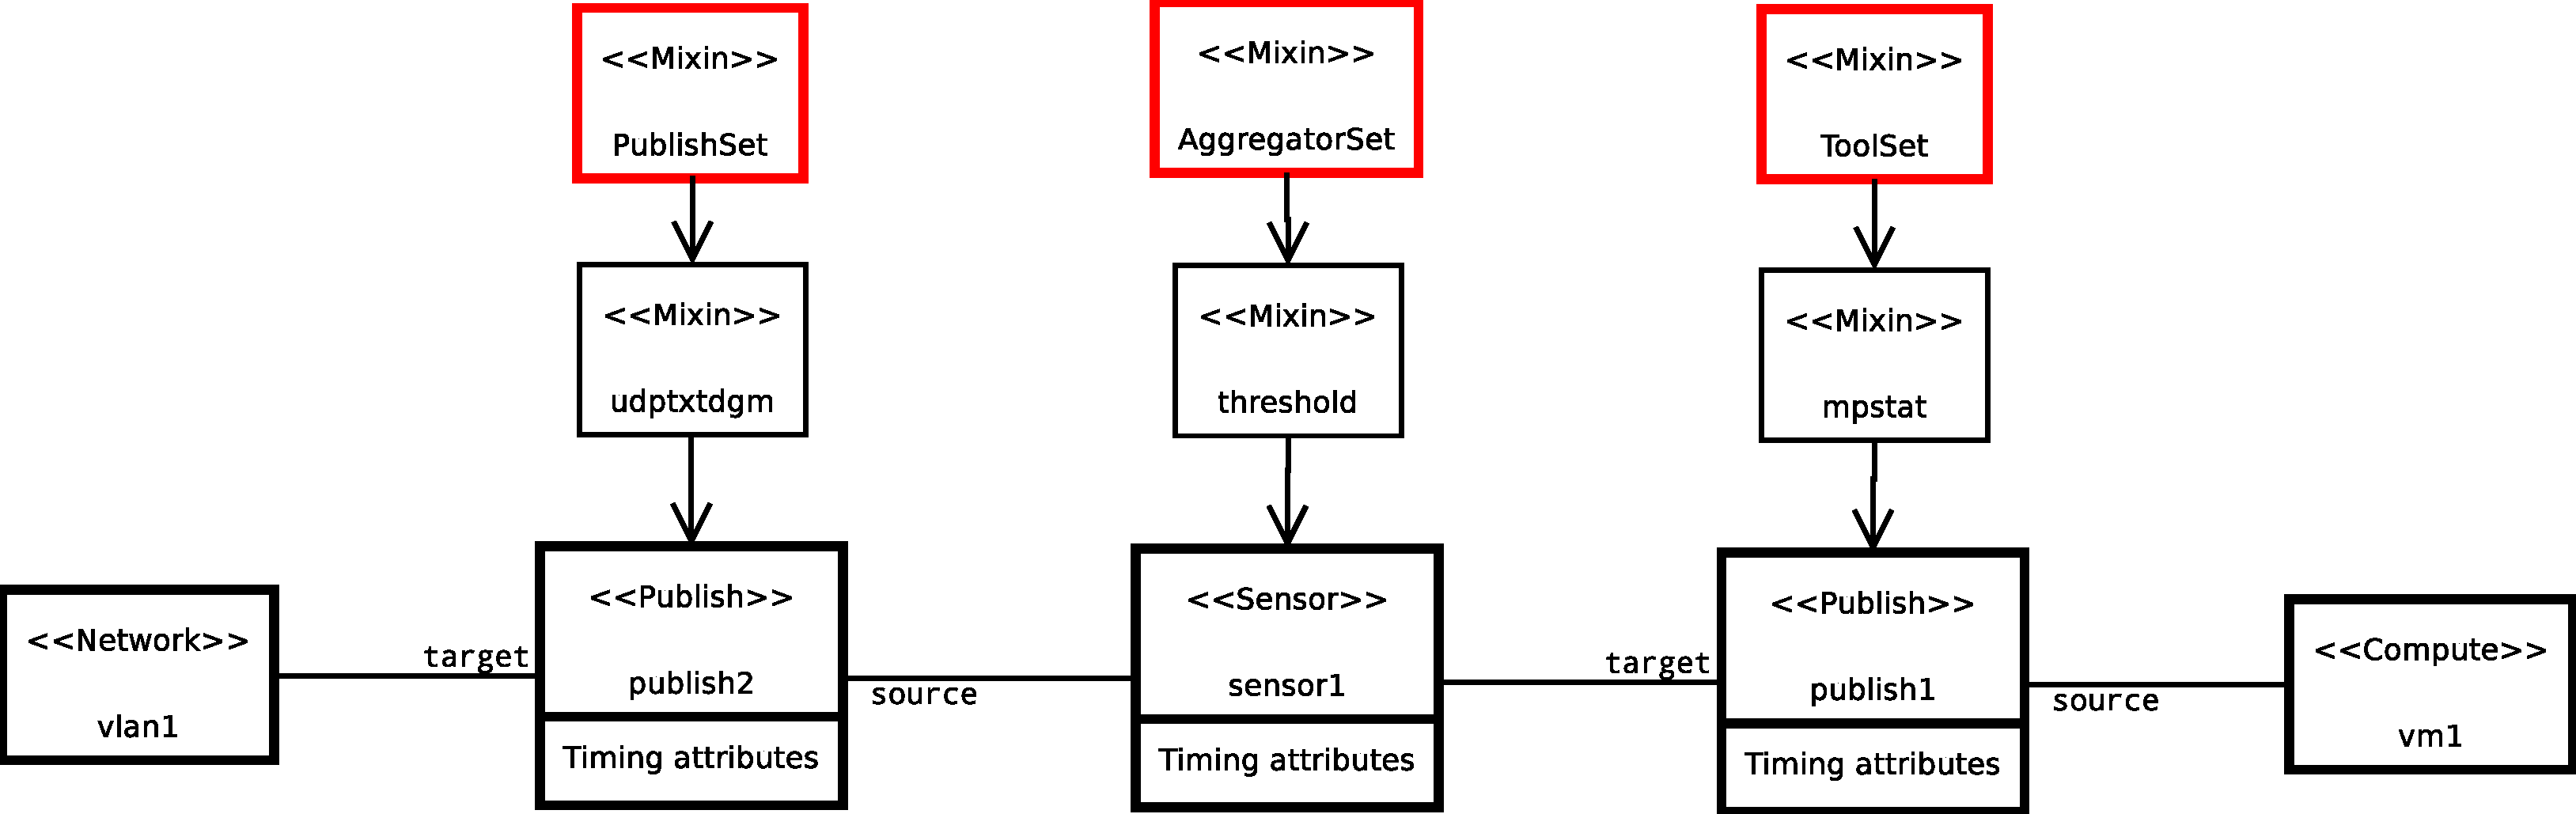
\includegraphics[width=\linewidth]{newDiagram_V3.pdf}
\caption{The instance diagram of the monitoring infrastructure \label{fig:example}}
\end{figure}

The user starts instantiating a new \sens, and a \coll\ connecting {\tt vm1} to the sensor. The new \sens:

\begin{verbatim}
> POST /sensor/ HTTP/1.1
> Category: sensor; 
            scheme:"http://schemas.ogf.org/occi/monitoring#"; 
            class="kind"
...
< HTTP/1.1 201 OK
< Location: "http://provider.com/monitoring/sensor1
\end{verbatim}

the input \coll:

\begin{verbatim}
> POST /collector/ HTTP/1.1
> Category: collector;
>           scheme="http://schemas.ogf.org/occi/monitoring#";
>           class="kind";
> X-OCCI-Attribute: occi.core.target="http://provider.com/monitoring/sensor1
> X-OCCI-Attribute: occi.core.source="http://provider.com/vms/vm1
> ...
...
< HTTP/1.1 201 OK
< Location: "http://provider.com/monitoring/collector1
\end{verbatim}

and the input \coll:

\begin{verbatim}
> POST /collector/ HTTP/1.1
> Category: collector;
>           scheme="http://schemas.ogf.org/occi/monitoring#";
>           class="kind";
> X-OCCI-Attribute: occi.core.target="http://provider.com/net/vlan1
> X-OCCI-Attribute: occi.core.source="http://provider.com/monitoring/sensor1
> ...
...
< HTTP/1.1 201 OK
< Location: "http://provider.com/monitoring/collector2
\end{verbatim}
The timing attribuites of the three instances are filled in

\begin{verbatim}
POST /monitoring/sensor1/ HTTP/1.1
> ...
> X-OCCI-Attribute: occi.sensor.period=10;
> X-OCCI-Attribute: occi.sensor.periodspec="1,0.1,1";
> X-OCCI-Attribute: occi.sensor.timestart=10
> X-OCCI-Attribute: occi.sensor.timestop=3600;
> X-OCCI-Attribute: occi.sensor.timegranularity="1,0.1,1";
\end{verbatim}

\begin{verbatim}
POST /monitoring/collector1/ HTTP/1.1
> ...
> X-OCCI-Attribute: occi.collector.period=10;
> X-OCCI-Attribute: occi.collector.periodspec="1,0.1,1";
\end{verbatim}

\begin{verbatim}
POST /monitoring/collector2/ HTTP/1.1
> ...
> X-OCCI-Attribute: occi.collector.period=10;
> X-OCCI-Attribute: occi.collector.periodspec="1,0.1,1";
\end{verbatim}

The monitoring activity will start in 10 seconds and last for 1 hour, performing one measurement every 10 seconds. Granularity and accuracy are just consistent with the timing requirements.

Next, the user browses the {\tt ToolSet} collection looking for a tool that measures processor idle time: the search pattern comes from outside our scenario. It finally finds {\tt mpstat}, defined as in table \ref{tab:mpstat} in the provider's namespace {\tt http://provider.com/monitoring/}.

\begin{table}
\scriptsize
\extramixin{mpstat}{(see table below)}

\attributes{mpstat \mi}{
com.provider.tool.port & number & true & true &  The port where to send a measurement trigger (control) \\
com.provider.tool.ncpu & number & false & true & The number of processors (metric) \\ 
com.provider.tool.idletimecpu & number & false & true & Total percent of idle time (metric)  \\ 
com.provider.tool.usertimecpu & number & false & true & Total percent of user time (metric) \\
com.provider.tool.systimecpu & number & false & true & Total percent of system time (metric) \\
}
\caption{Attributes defined for the {\tt mpstat} mixin \label{tab:mpstat}}
\end {table}

Then it associates {\tt link1} with the {\tt mpstat} \mi:

\begin{verbatim}
> POST /toolset/mpstat/ HTTP/1.1
> X-OCCI-Location: http://provider.com/monitoring/collector1
\end{verbatim}

This latter operation is critical, and may give rise to a number of errors, that result in 4xx and 5xx error codes. For instance, the server may return {\tt 403 Forbidden} in the case the {\tt ToolSet} \mi\ is not legal for the target resource.

In the general case, the above steps are repeated for every metric that the user needs to measure to compute the application-denpendent metric. Here we proceed to the next step. 

The user now searches a \mi\ in the {\tt AggregatorSet} collection that returns a threshold signal: it finds the {\tt Threshold} defined in table \ref{tab:vat}

\begin{table}
\scriptsize
\extramixin{threshold}{(see table below)}

\attributes{threshold}{
com.provider.sensor.threshold & number & true & true & The threshold value (control) \\
com.provider.sensor.mode & {Once,Continuous} & true & true & How frequent the warning message (control) \\ 
com.provider.sensor.fallmsg & String & true & true & The falling edge message \\
com.provider.sensor.risemsg & String & true & true & The rising edge message \\
com.provider.sensor.input & URI & false & true & The input value (input)  \\  
}
\caption{Attributes defined for the {\tt threshold} mixin \label{tab:vat}}
\end {table}

The next step of the user is to associate the \sens\ to the \mi,

\begin{verbatim}
> POST /computetool/threshold/ HTTP/1.1
> ...
> X-OCCI-Location: http://provider.com/monitoring/sensor1
\end{verbatim}
 
and fills in the attributes as appropriate:

\begin{verbatim}
POST /monitoring/sensor1/ HTTP/1.1
> ...
> X-OCCI-Attribute: com.provider.sensor.threshold=10
> X-OCCI-Attribute: com.provider.sensor.mode="Once"
> X-OCCI-Attribute: com.provider.sensor.fallmgs="Warning: vm1 overloaded"
> X-OCCI-Attribute: com.provider.sensor.risemgs="vm1 load below 90%"
> X-OCCI-Attribute: com.provider.sensor.input="com.provider.monitoring.tool1.idletimecpu"
\end{verbatim}

The server here responds with a {\tt 404 Not found} if the {\tt input} attribute does not exist, or {\tt 401 Unauthorized} if the user is not allowed to operate on that \rs\ (e.g., the metric is outside its scope).

Finally the user associates a way to publish the result: a UDP datagram on a network. It looks in the {\tt CollectorSet} collection the \mi\ that applies, and finds the one described in figure \ref{tab:udp}, that sends a string as a UDP datagram.

\begin{table}
\scriptsize
\extramixin{udptxtdgm}{(see table below)}

\attributes{udptxtdgm}{
com.provider.sensor.dest & String & true & true & The destination of the message (control) \\
com.provider.sensor.port & number & true & true & The destination port (control) \\ 
com.provider.sensor.mode & {all,nonempty} & true & true & Indicate whether only non empty msg are sent (control) \\ 
com.provider.sensor.input & URI & true & true & The msg to be sent \\
}
\caption{Attributes defined for the {\tt udptxtdgm} mixin \label{tab:udp}}
\end {table}

It then associates that \mi to the outgoing \coll:

{\scriptsize
\begin{verbatim}
> POST /collectorset/udptxtdgm/ HTTP/1.1
> ...
> X-OCCI-Location: http://provider.com/monitoring/collector2
\end{verbatim}
 }
and fills in the attributes as appropriate:

\begin{verbatim}
POST /monitoring/collector2/ HTTP/1.1
> ...
> X-OCCI-Attribute: com.provider.schema.destination="ctr1.provider.com";
> X-OCCI-Attribute: com.provider.schema.port="10222";
> X-OCCI-Attribute: com.provider.schema.mode="nonempty";
> X-OCCI-Attribute: com.provider.schema.input="http://provider.com/monitoring/sensor1/compoutput";
\end{verbatim}

%!TEX root = nml-base.tex

\section{Intellectual Property Statement}

The OGF takes no position regarding the validity or scope of any intellectual property or other rights that might be claimed to pertain to the implementation or use of the technology described in this document or the extent to which any license under such rights might or might not be available; neither does it represent that it has made any effort to identify any such rights.  Copies of claims of rights made available for publication and any assurances of licenses to be made available, or the result of an attempt made to obtain a general license or permission for the use of such proprietary rights by implementers or users of this specification can be obtained from the OGF Secretariat.

The OGF invites any interested party to bring to its attention any copyrights, patents or patent applications, or other proprietary rights which may cover technology that may be required to practice this recommendation.  Please address the information to the OGF Executive Director.

\section{Disclaimer}

This document and the information contained herein is provided on an ``As Is'' basis and the OGF disclaims all warranties, express or implied, including but not limited to any warranty that the use of the information herein will not infringe any rights or any implied warranties of merchantability or fitness for a particular purpose.

\section{Full Copyright Notice}

Copyright \copyright \ Open Grid Forum (\copyrightyears). Some Rights Reserved.

This document and translations of it may be copied and furnished to
others, and derivative works that comment on or otherwise explain it
or assist in its implementation may be prepared, copied, published and
distributed, in whole or in part, without restriction of any kind,
provided that the above copyright notice and this paragraph are
included as references to the derived portions on all such copies and
derivative works. The published OGF document from which such works are
derived, however, may not be modified in any way, such as by removing
the copyright notice or references to the OGF or other organizations,
except as needed for the purpose of developing new or updated OGF
documents in conformance with the procedures defined in the OGF
Document Process, or as required to translate it into languages other
than English. OGF, with the approval of its board, may remove this
restriction for inclusion of OGF document content for the purpose of
producing standards in cooperation with other international standards
bodies.

The limited permissions granted above are perpetual and will not be
revoked by the OGF or its successors or assignees.


% \phantomsection\addcontentsline{toc}{section}{References}
\section{References}

% Define heading of bibliography to be empty, since we already have a heading above the text.
\renewcommand{\refname}{}
\vspace*{-3em}

% Use bibliography.bib for references.
\bibliography{biblio,cur}

% Alternatively, you can insert the bibliography inline, like so:
% 
% \begin{thebibliography}{5}
% 
% \bibitem[GFD0000()]{gfd0000}
% Firstname Author1 and Firstname Author2.
% \newblock {Our Awesome Grid Forum Document}.
% \newblock GWD-C.0000, April 2002.
% 
% \bibitem[GFD152()Catlett, de~Laat, Martin, Newby, and Skow]{gfd152}
% Charlie Catlett, Cees de~Laat, David Martin, Gregory~B. Newby, and Dane Skow.
% \newblock {Open Grid Forum Document Process and Requirements}.
% \newblock GFD-C.152, June 2009.
% \newblock URL \url{http://www.ogf.org/documents/GFD.152.pdf}.
% 
% \bibitem[RFC2119()]{rfc2119}
% Scott Bradner.
% \newblock {Key words for use in RFCs to Indicate Requirement Levels}.
% \newblock RFC 2119 (Best Current Practice), March 1997.
% \newblock URL \url{http://tools.ietf.org/html/rfc2119}.
% 
% \bibitem[RFC3552()Rescorla, Korver, and {Internet Architectures Board}]{rfc3552}
% Eric Rescorla, Brian Korver, and {Internet Architectures Board}.
% \newblock {Guidelines for Writing RFC Text on Security Considerations}.
% \newblock RFC 3552 (Best Current Practice), July 2003.
% \newblock URL \url{http://tools.ietf.org/html/rfc3552}.
% 
% \bibitem[RFC3967()]{rfc3967}
% Randy Bush and Thomas Narten.
% \newblock {Clarifying when Standards Track Documents may Refer Normatively to Documents at a Lower Level}.
% \newblock RFC 3967 (Best Current Practice), December 2004.
% \newblock URL \url{http://tools.ietf.org/html/rfc3967}.
% 
% \end{thebibliography}



\end{document}
